\documentclass[11pt,a4paper,oneside]{article}
\renewcommand{\baselinestretch}{1.2}
\usepackage{sectsty,setspace,natbib,wasysym} 
\usepackage[top=1.00in, bottom=1.0in, left=1in, right=1.25in]{geometry} 
\usepackage{graphicx}
\usepackage{latexsym,amssymb,epsf} 
\usepackage{epstopdf}
\usepackage{exceltex}
\usepackage{amsmath}
\usepackage{natbib}


\usepackage{fancyhdr}
\pagestyle{fancy}
\fancyhead[LO]{August 2012}
\fancyhead[RO]{Variable environments \& climate change}

\begin{document}
\renewcommand{\labelitemi}{$ $}
\title{Coexistence and climate change: \\The role of
    temporal-variability in structuring future communities}
    \author{Wolkovich, Donahue . . .}
\date{Last updated: 17 August 2012}
\maketitle
\noindent {\Large Lizzie! Finish writing up all your August 2012 notes soon! That includes re-doing the dimensional analysis neatly and scanning any important notes!}

\begin{abstract} Predicting community shifts
with climate change requires fundamental appreciation of the
mechanisms that govern how communities assemble. Most work to date has
focused on how warmer mean temperatures may affect individual species
via physiology, generally producing range shifts towards the poles and
uphill, which fails to predict the wide diversity of observed shifts.
Climate change has and is expected to affect far more than mean
temperatures, including widespread affects on growing season
length, variability and shifts in extreme events. Additionally,
cascading effects on species and communities are qualitatively
predicted but there have been no efforts, to our knowledge, to predict
shifts based on coexistence theory. Here we extend the two possible
mechanisms for species coexistence based on variable environments---
relative nonlinearity and the storage effect---to predict how
communities will respond to climate change. We focus on both (1) shifts in
climate variability and extreme events that link to
stabilizing coexistence mechanisms and (2) traits that may
make species the most vulnerable to climate change. Specifically we examine how
synergistic effects of climate on multiple abiotic variables---for
example, earlier precipitation pulses and higher evapotranspiration
associated with earlier snowpack melting in the Sierras---alter
coexistence compared to single, unlinked variables. We then examine how
coexistence outcomes under shifting climate regimes vary with the
ability of species to track the timing of major climate events. \emph{We
  (might) find out that synergistic effects of multiple shifting
  abiotic variables reduce coexistence greater than single
  variables. Species that can track variability are least vulnerable
  to climate change (perhaps).  Also, we add an emphasis on integrating intra and inter-annual
scales here, if we manage to make that happen well.}
\end{abstract}

\newpage

\section{Next steps, fall 2012 goals!}
\noindent {\bf \emph{Was} September-October 2011 goals, ohbother}\\
\\
\noindent We have Matlab and R code running the model as a 2 species
(we decided to start here, and then debate whether and how to extend
to a more diverse community, but the code is in matrix format so the
mechanics, if not the concepts and results, will be easy to extend) but we need
to:
\begin{enumerate}
\item Check that it's running well and time-scales issues (intra- to
  inter-annual variability) are handled well. {\bf Megan} needs to do
  this, including deciding if we need to ODE solve the intra-annual
  dynamics, then use the discretized version only inter-annually. Note from Lizzie: best ODE solver is now in package `desolve.'
\item{\bf Soon!:} Lizzie needs to clean up notes on dimensions and re-do dimension analysis given table 1 here.
\item{\bf Soon!:} Megan needs to update this with new equation for phenological tracking.
\end{enumerate}

\section{Introduction}
\noindent \emph{Need to write more someday} \\
\noindent Understanding how plant communities will respond to climate change
requires synthesizing information on both direct effects of climate on species
and indirect effects driven by responses to other species'
shifts. (Coexistence models based on variable environments allow us to
do this, as species respond to shifting resources, which are
influenced both by abiotic stressors and the use of the resource by
other species.)

\section{Overview of project and directions}
\noindent After the July 2011 meeting there are a couple major
angles to this paper. I am not sure one has been picked yet, but one needs to pick up center stage
someday and the others fall behind.
\begin{enumerate}
\item We consider the effects of climate variation at both the
intra-annual and inter-annual scale and scale up responses to
short-term (1-10 yr?) and long-term (\(>\)100 yr) dynamics. 
\item We compare the compounding effect of climate change: examining
  how shifts in single versus multiple environmental variables affect
  coexistence.
\item We also look at how species traits related to their responses to
  climate variability effect coexistence and long-term diversity
  maintenance. (This is the tracking part of the project.) 
\end{enumerate}
As of July 2011 I would say that the greatest interest in setting up
the paper lied in focusing on single vs. multiple variables, then
putting in tracking as subordinate. \\
\\
\noindent We also note that one possible way to make this project more
interesting, useful and forward-thinking than others is to make
scenarios most realistic---link to real climate scenarios or use
existing data to rule out and in shifts in abiotic variables (and
possibly species traits---we should have the data to estimate the
percentage of species that track, maximum tracking and if only
early-season species track, we could add that in, and of course we
have a lot of climate data on hand).

\section{Current outline}
\begin{enumerate}
\item Introduction
\begin{enumerate}
\item Direct and indirect effects of climate change
\item Links to ecological coexistence theory
\item Abiotic shifts expected with climate change: single versus
  synergistic climate shifts
\item Things that will shift with climate change, related to
  coexistence models
\begin{enumerate}
\item Magnitude of and interannual variance in resource pulse (\(R_{\theta}\))
\item Timing of resource pulse (\(\tau_{p}\))
\item Abiotic loss rate of resource (\(\epsilon\))
\end{enumerate}
\item Species traits and climate change: phenological tracking
\item Goals of paper
\end{enumerate}
\item Model description (a whole section on this below)
\begin{enumerate}
\item Basic storage effect model
\item Our version of the storage effect model
\item Systems for which model is applicable: This is effectively a system with a single large pulse of
resource, that, in a plant-free scenario is lost exponentially each
year. 
\begin{enumerate}
\item Alpine systems (resource is water): initial large pulse of precipitation from
  snowpack that gradually is used up  throughout season
\item Arid systems? (resource is water): Major pulse of rains (okay, spread out some,
  but really they often concentrate for a couple months and then
  season continues for 3-4 more months)
\item Temperate systems (resource is nutrients): Work with me here, I
  think this is cool. Early in the season turnover of microbes leads
  to a huge flush of nutrients \citep{Zak:1990ar} that microbes (and plants) draw down
  all season. There's no other pulse really---am I crazy here or
  doesn't this work well? (And so microbes draw it down in the
  plant-free case which could easily be affected by climate change,
  e.g., increased temperatures lead to increased microbial activity
  and more rapid draw-down.)
\end{enumerate}
\item Systems it probably doesn't work for: Light-limited systems
  (there is not a single, plant-free decreasing pulse of resource),
  Great Plains or others with multiple pulses.
\item Phenological tracking and the storage effect
\item Our implementation of tracking
\item Derivation of aspects of the storage effect and relative
  non-linearity in our model (this is a big \emph{to do}).
\end{enumerate}
\item Results: (response variables are (1) probability of extinction,
  (2) relative
  densities in 2 spp models)
\begin{enumerate}
\item Section 1: Shifting abiotic variables, single versus co-varying
  shifts 
\item Section 2: Species traits: Phenological tracking and shifting
  abiotic variables
\end{enumerate}
\item Discussion
\end{enumerate}

\section{Variables of interest}
\noindent We
consider 2 primary traits of the environment (\(\epsilon, R\), which
code to evaporative stress and inter-annual variability for our approach basically) and 1
species response trait (phenology, specifically flexibility in
phenology as modeled by a species' ability to shift \(\tau_{i}\)) to model
the dominant expectations of current and future climate change:
\begin{enumerate}
\item \emph{Changes to R:} Shifts in climate means and variability (greater var \(\approx\)
  extreme events) as modeled by changes to \(\mu\) and \(var\) of
    R,
  which can lead to:
\begin{enumerate}
\item Changes to relative non-linearity (shifts on the X axis due to
  new extremes etc.)
\item Changes in inter-annual covar(E, C)
\item For variability: changes related to buffered population growth:
  for example, when the periodicity of certain extreme events declines
  such that species with certain buffering times no longer get their
  `good' years enough (e.g., periodicity of rainy years every 5 years,
  switches to 10 and the species seedbank is 7 years). This means for
  simulations changing \(var(R)\) must be consider in concert with the
  scale of \(s_{i\cdots n}\).
\end{enumerate}
\item \emph{Changes to \(\epsilon\):} Shifts in climate means that lead to greater abiotic stress on
  environments, as modeled by changes to  \(\epsilon\). For example,
  warmer growing seasons may produce greater evapotranspiration,
  shifting competition for the remaining resource. (By the way, we
  have notes about treating \(\epsilon\) as a function itself.) This should
  affect:
\begin{enumerate}
\item Changes to relative non-linearity
\item Changes in inter-annual covar(E, C)
\end{enumerate}
\item \emph{Changes to \(\tau\):} Longer growing seasons, with several scenarios:
\begin{enumerate}
\item Season is longer (earlier \(\tau_{p}\) but community of species
  do not shift their timing (e.g., no change to  \(\tau_{i \cdots
    n}\)) 
\item Season is longer (earlier \(\tau_{p}\) and some species (`climate-trackers') change
  their timing (community shift in temporal (phenological) synchrony),
  that is (e.g., certain species change to  \(\tau_{i \cdots
    n}\)) such that the distance \(\tau_{p}-\tau_{i}\) is constant
  across years.
\item Could also look at complementarity (histogram of variation in \(\tau_{i \cdots
    n}\); could pull \(\tau_{i \cdots
    n}\) from a beta distribution. (Note: I also wonder if we
  shouldn't just use variation due to above to look at this, versus a
  whole new approach.)
\end{enumerate}
\item How do these variables shift with climate change and co-vary?
\begin{enumerate} 
\item \(R_{\theta}\) increasing inter-annual variance with some giant
  years (extreme events), for snowpack systems it's decreasing
  generally
\item \(\tau_{p}\) getting earlier, also for snowpack systems earlier
  years probably also have higher evaporative stress (\(\epsilon\),
  due to warmer year)
\end{enumerate}
\end{enumerate}
\\
\noindent We assume that:
\begin{enumerate}
\item All species `go' each year, at least a little; that is, we're
  not looking at a communities where some species have true
  supra-annual strategies.
\item There is one dominant pulse of the limiting resource (e.g.,
  light or water) at the
  start of each growing season; thus we model a  single pulse per
  season.
\item While interactions between the above-considered `traits' may be
  important, first understanding how each of these forces act alone is
  critical enough to let alone interactions for this manuscript.
\end{enumerate}
\\
\noindent We also discussed mucking with \(m_{i}\) (the partial
mortality of species) to play around with
shifts in extreme events such as more frost dates following spring
warmth. But the above is more well-demonstrated or expected as
climate-related issues so we're not going there. (Note from Lizzie in
July 2011: I think this topic will be cool someday as it might be a
real issue in subalpine communities, but for now it's not for
sure. And given the equations we're using, it's not as crisp as the
above to get from \(environment\rightarrow m_{i}\).)
\\


\noindent {\bf Some notes for writing}
\begin{enumerate}
\item Understanding the variable responses of communities and species
  due to climate shifts is a major aim of current
ecology.
\begin{enumerate}
\item Varied responses
\begin{enumerate}
\item reversed phenology \citep{yu2010} 
\item downhill shifts \citep{Crimmins:2011dq}
\end{enumerate}
\item Effects of climate change extend well beyond shifts in the mean
\end{enumerate}
\item Models of community assembly in ecology build upon coexistence
  via environmental variability.
\item Launch into set-up.
\end{enumerate}
\noindent Some key refs we worked with:
\citep{Chesson:1993gi,Chesson:2000ak,Chesson:2000vd,Chesson:2004eo}. Some
papers using storage effect model or Armstong and McGhee with field
data: \citep{Angert:2009ng,Kuang:2008ri,Kuang:2009rj,Levine:2009ym}.
\\
\\
\noindent The way the growing season ends in the equations is
interesting. First, as brilliantly stated: the growing seasons ends
[in these equations] when plants stop growing. And related, the
equations do not deal with setting the end of the growing season. In
my head (Lizzie), abiotic forces can stop a growing season, but in
reality with plant phenology data, the start and end of the growing
season are fundamentally different: at the start species are most
sensitive to abiotic cues and climate change effects are large and
often consistent. For the end of the season effects have been more
muted and variable---suggesting plants in someway do seem to set the
end of the growing season more than abiotic cues do, at least when
compared to the start of season. (And the model follows this.)
\\
\\
\noindent The 3 ingredients of the storage effect are:
\begin{enumerate}
\item differential response to the environment (subadditivity)
\item covar(E, C)
\item buffered population growth
\end{enumerate}

\section{Little things done and to do:}
\begin{enumerate}
\item Done:
\begin{enumerate}
\item In August 2012 Megan came up with a new way to model phenological tracking, it's linear and better than the one presented here. We also discussed three key ways to think of tracking:
\begin{enumerate}
\item Species can have fixed flowering/leafing (not track).
\item Species can phenological track pulse.
\item Species can phenological track something at least at one time in history correlated with the pulse.
\end{enumerate}
We agreed that while (3) is interesting---would allow you to look at mismatch ideas etc.---(1) and (2) have more biological support for plants and are interesting enough in and of themselves, so we will focus on and mode (1) and (2) and not (3).
\item In July 2011, I looked at whether the start of spring
has gotten more variable (using some key datasets from NECTAR) and it
hasn't, at all. No change.
\item  Have looked twice now at who has cited Chesson et al. 2004
and for actual modeling work it's just Chesson, and for that it's all
his seed predation work.
\item The intra-annual model does not have a useful closed solution (I
  have some Maxima code that shows only the trivial solution gives an
  equilibrium). This actually makes sense since the model is not a
  chemostat (a la Tilman \(R^{*}\)), we have a pulse that drains out
  and is not balanced by inputs.
\end{enumerate}
\item To do (Lizzie):
\begin{enumerate}
\item Get on top of climate change lit: which variables will shift?
  Which ones are coupled and how will their coupling shift with
  climate change (go from uncoupled to coupled, or vice-versa, or just
  the coupling itself changes). 
\item Does evaporative stress increase with climate change (absolute,
  versus relative, oceans burn off while temperatures increase etc.)
\item When seasons start earlier does evaporative stress increase (I
  suspect so, but need to pull together refs)
\item Does lower snowpack mean earlier seasons?
\end{enumerate}
\end{enumerate}

\section{Scratch notes from August 2012}
\begin{itemize}
\item  Issue we worried about: Will tracker always win? Answers: No, not if it's a poor competitor, that is, if it responds quickly but does poorly at low resource levels. I also think it's important to remember that not all tracking species will track perfectly so some species should grow before trackers some years, when their fixed \(\tau_{i}\) corresponds well to \(\tau_{p}\). Also, we have a note high intraspecific competition could dampen trackers, especially when greater than interspecific competition.
\item . . . 
\item I need to enter the rest soon.
\end{itemize} 

\newpage
\section{Equations and related notes}

\noindent For a species \(i\) let:
\begin{align*}
N_{i} & \text{   seedbank of species } i
\\
s_{i} & \text{   survival of seedbank of species } i \text{, buffered pop'ln
  growth occurs via this constant}
\\
\delta & \text{   total time of growing season}
\\
B_{i} &  \text{   biomass of species } i
\\
R &   \text{   resource}
\\
f_{i}(R) & \text{  resource uptake rate of species } i \text{ of } R
\\
c_{i} & \text{   conversion of uptake to biomass of species } i
\\
m_{i} & \text{   partial mortality of species } i
\\
a_{i} & \text{   uptake increase for species } i \text{ as R increases}
\\
\theta_{i} & \text{   shape of uptake of species } i
\\
d_{i}^{-1} & \text{   max uptake of species } i
\\
G_{i} & \text{   max germination of species } i
\\
h_{i} & \text{   max rate of germination decrease of species } i
\text{ following a pulse}
\\
\tau_{p} & \text{   time of pulse }
\\
\tau_{i} & \text{   time of max germination of species } i
\\
\epsilon & \text{   abiotic loss of resource}
\\
\phi_{i} & \text{   conversion of biomass of species } i \text{ to
  seedbank}
\\
b_{i} & \text{   seedling biomass of species } i
\\
\alpha & \text{   phenological tracking of species  } i
\\
\end{align*}

\newpage
\noindent System of equations, for a community of \(n\) species based
on resource competition:
\begin{align*}
N_{i}(t+1) & = N_{i}(t+\delta)s_{i}
\\
\\
& \text{where}
\\
\\
N_{i}(t+\delta) & = N_{i}(t) [\text{germination fraction}][\text{seeds
  produced per germinant}]
\\
\\
& \text{so then:}
\\
\\
N_{i}(t+1) & =
s_{i}(N_{i}(t)(1-g_{i})+N_{i}(t)g_{i}\phi_{i}\int_t^{t+\delta}[c_{i}f_{i}(R(t))-m_{i}]B_{i}(t)\mathrm{d}t)
\\
\\
\frac{\mathrm{d}R}{\mathrm{d}t} & = - \sum_{i=1}^{n}f_{i}(R)B_{i} -\epsilon R
\\
\\
\frac{\mathrm{d}B_{i}}{\mathrm{d}t} &  = [c_{i}f_{i}(R) - m_{i}]B_{i}
\\
\\
& \text{where:} 
\\
\\
g & = G_{i}e^{-h(\tau_{p}-\tau_{i})^2}
\\
\\
f_{i}(R) & = \frac{a_{i}R^{\theta_{i}}}{1+a_{i}d_{i}R^{\theta_{i}}}
\\
\end{align*}
\noindent Adding phenological tracking to the model:
\begin{align*}
\hat{\tau_{i}} & = \tau_{p}-(\tau_{p}-\tau_{i})e^{-\alpha}
\end{align*}
\noindent thus, when:
\begin{align*}
& \alpha=0, \hat{\tau_{i}}=\tau_{i}
\\
& \alpha=\infty, \hat{\tau_{i}}=\tau_{p}
\end{align*}

\noindent Getting this into simulation-landia means:
\begin{align*}
B_{i}(0) & = [\text{number of seeds}][\text{germination
  fraction}][\text{seedling biomass}]
\\
\\
\text{which also looks like:}
\\
\\
B_{i}(0) & = N_{i}(t) g_{i}b_{i}
\\
\\
B_{i}(t+\mathrm{d}t) & =B_{i}(t)+[c_{i}f_{i}R(t)-m_{i}]B_{i}(t)\mathrm{d}t
\end{align*}
\\
\\
\noindent Also note that I made one change from the February 2011 board: I think we
used \(h\) accidentally twice for different meanings: one was in the
equation for \(g_{i}\) which we stole from \cite{Chesson:2004eo}
(appendix, see next note), and then one was for the total length of time for the
growing season. Thus I changed this `season-length' \(h\) to
\(\delta\).
\\
\\
\noindent Finally, equations for \(\frac{dB_{i}}{dt}, f_{i}R, g_{i},
\frac{dR}{dt}\) were taken from the appendix of \cite{Chesson:2004eo} (\emph{Oecologia}).

\newpage 
\noindent {\bf Dimensional analysis}\\
\noindent \emph{Exciting new product as of August 2012, oh la la!}
\\
\begin{center}
\begin{table}[h!]
\caption{Table of parameter values, their definitions and lightweight version of their dimensions (i.e., not yet deemed `grams' or such).}
\begin{tabular}{ | p{3.0cm} | p{6.0cm} | p{4.0cm} |}
\hline 
Parameter & Definition & Unit \\ \hline 
\end{tabular}
\begin{tabular}{ | p{3.0cm} | p{6.0cm} | p{4.0cm} |}
\(N_{i}\) & seedbank of species \(i\) & seeds \\ \hline
\(s_{i}\) & survival of species \(i\) & unitless \\ \hline
\(\delta\) & total length of growing season & days\\ \hline
\(B_{i}\) & biomass of species \(i\) & biomass \\ \hline
\(R\) & resource & resource\\ \hline
\(f_{i}\) & resource uptake rate &  \(\frac{\text{resource}}{(\text{days})(\text{biomass})}\)\\ \hline
\(c_{i}\) & conversion of \(R\) uptake to biomass of species \(i\) &  \(\frac{\text{biomass}}{\text{resource}}\) \\ \hline
\(m_{i}\) & maintenance costs of species \(i\) & \(\text{days}^{-1}\) \\ \hline
\(a_{i}\) & uptake increase as \(R\) increases for species \(i\) & \(\text{days}^{-1}\) \\ \hline
\(d_{i}\) & max uptake for species \(i\) & \(\frac{(\text{days})(\text{biomass})}{\text{resource}}\) \\ \hline
\(\phi_{i}\) & converesion of biomass to seedbank for species \(i\) & \(\text{biomass}^{-1}\), but conceptually \(\frac{\text{seeds}}{(\text{biomass})(\text{seeds})}\) \\ \hline
\(\epsilon\) & abiotic loss of \(R\) &  \(\text{days}^{-1}\) \\ \hline
\(G_{i}\) & max germination of species \(i\) & unitless \\ \hline
\(h_{i}\) & max germination of species \(i\) following \(R\) pulse & \(\text{days}^{-2}\) \\ \hline
\(g_{i}\) & germination fraction & unitless \\ \hline
\(\tau_{p}\) & timing of pulse & days \\ \hline
\(\tau_{i}\) & timing of max germination of species \(i\) & days \\ \hline
\(\alpha_{i}\) & phenological tracking of species \(i\) & unitless \\ \hline
\(\theta_{i}\) & shape of uptake for species \(i\) & unitless\\ \hline
\hline
\(b_{i}\) & seedling biomass of species_{i} & \(\frac{\text{biomass}}{\text{seeds}}\) \\ \hline
\(f_{i}(R)\) & \(R\) uptake \(f(x)\) for species \(i\) & \(\frac{\text{resource}}{(\text{days})(\text{biomass})}\)\\
\hline
\end{tabular}
\end{table}
\end{center}


\newpage
\noindent {\bf Some random notes from the whiteboard:}\\
\noindent Relative nonlinearity is:
\begin{align*}
\left(\frac{d^{2}}{dR^{2}}\right)(var(R))
\end{align*}
\noindent Non-additivity (\(\gamma\)) is (in general, still working on
what it is for our equations) when considering population growth
(\(r_{i}\)):
\begin{align*}
r_{i} & = \omega_{i}(E_{i}, C)
\\
\\
\gamma & = \frac{\partial \omega}{\partial E \partial C} 
\end{align*}

\noindent but, what is \(E\) and \(C\) in our system?
\begin{align*}
C & = - \sum_{i=1}^{n}f_{i}(R)B_{i} \rightarrow f_{i}R
\end{align*}
\noindent is this (above) the response to
  competition? An alternative note we had with many question marks
  was:
\begin{align*}
covar(E,C) \approx covar\left(R_{i}, \sum_{i=1}^{n}B_{i}\right)
\end{align*}

\newpage
\bibliography{/Users/Lizzie/Documents/git/bibtex/LizzieMainMinimal}
\bibliographystyle{/Users/Lizzie/Documents/git/bibtex/styles/ecolett.bst}

\newpage
\begin{figure}[h!]
\centering
\noindent 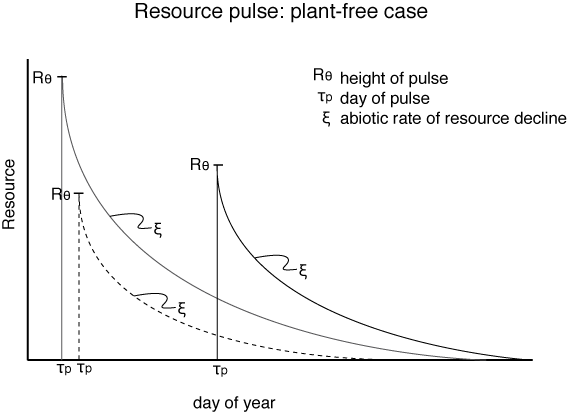
\includegraphics[width=0.8\textwidth]{/Users/Lizzie/Documents/git/temporalvar/figures/varenv_varying.png}
\caption{{\bf Major coexistence variables directly affected by
    climate change}  We focus on three major coexistence variables
  that have been (or will be) influenced by climate change---a couple
  examples of how varying them changes the resource pulse (without plants).}
\end{figure}

\newpage
\begin{figure}[h!]
\centering
\noindent 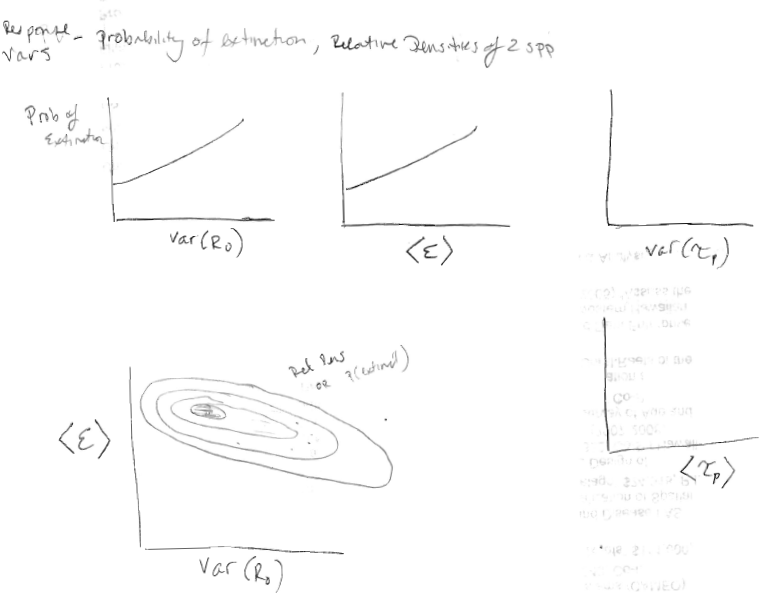
\includegraphics[width=1\textwidth]{/Users/Lizzie/Documents/git/temporalvar/figures/figurehopes_1.png}
\caption{{\bf Synergistic environmental effects.}  Figure aspirations
  for part 1 of the paper, which covers how varying environmental
  variables (\(\tau_{p}\), \(R_{\theta}\), \(\epsilon\)) alone and in concert (as predicted by climate change)
  alters coexistence. Single variables will be simple graphs, while
  contour plots will come in for varying more than one variable
  together. (There is no phenological tracking by species in this
  section of the paper.)}
\end{figure}

\newpage
\begin{figure}[h!]
\centering
\noindent 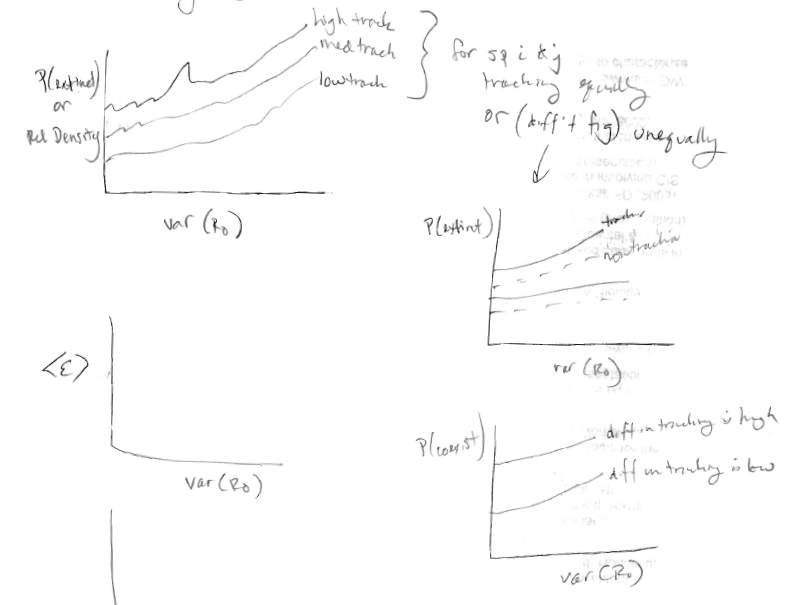
\includegraphics[width=1\textwidth]{/Users/Lizzie/Documents/git/temporalvar/figures/figurehopes_2.png}
\caption{{\bf Phenological tracking and coexistence under climate
    change.}  We didn't quite nail these down: do we vary both species
so they both track or look at one tracking and one not tracking?
Hoping this will become clear as we get the model up and running.}
\end{figure}

\end{document}